%!TEX root = ../report.tex

\section{Introduction}
Terminology:
\begin{description}
  \item[Protocols] control sending and receiving of messages
  \item[Internet] loosely hierarchical global network
  \item[Internet Standards]
    \begin{itemize}
      \item RFC:\@ Request for comment
      \item IETF:\@ Internet Engineering Task Force
      \item IANA:\@ Internet Assigned Numbers Authority
    \end{itemize}
\end{description}

\subsection{Protocols}
Protocols take care of addressing, fragmentation \& re-sequencing, error control, congestion control, compression, privacy and more.

The internet has an layered architecture of protocols.
On the sender side, protocols take the PDU (Protocol Data Unit) from layer N+1, add their header and trailer and pass the SDU (Service Data Unit) to layer N-1.
On the receiver side, the corresponding protocol takes the PDU from layer N-1, strips header and trailer again and passes the SDU to layer N+1.
\begin{figure}[H]
  \centering
  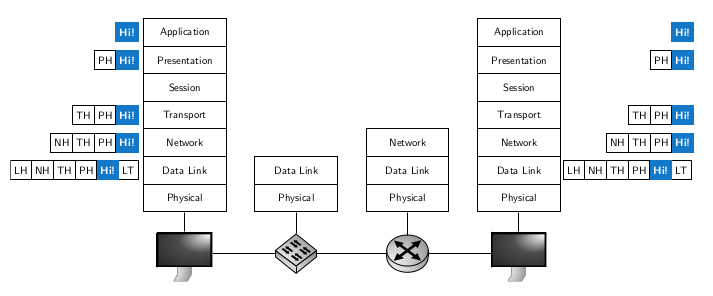
\includegraphics[width=.6\textwidth]{figures/internet_layering.png}
  \caption{Internet Layers}
\end{figure}

Protocol layering is necessary because one does not want to implement everything to the physical layer when writing a networking application.
On the other hand, layering also introduces some problems like protocol layers are sometimes reusing techniques of other layers like ARQ (Automatic Repeat Query) and layers might need informations of other layers.

\subsection{Node Forwarding Performance}
During transmission, packets might get delayed or even lost for several reasons.
First, the packets need some time to get written to router buffers, secondly the packet arrival rate might exceed the output link capacity and lastly the packets need to wait again for being sent from the packet queue in routers.

The sources for these delays are listed below.
\begin{enumerate}
  \item Processing delay: interrupt handling when receiving new packets and processing for further transmission
  \item Queuing delay: waiting time in output queue
  \item Transmission delay: time to send bits into link: $= \frac{\text{packet length L (bit)}}{\text{link bandwidth (bps)}}$
  \item Propagation delay $=\frac{\text{length of physical link d}}{\text{propagation speed} \approx 2 \cdot 10^8 m/s}$
\end{enumerate}
The total amount of delay is then $d_{nodal} = d_{proc} + d_{queue} + d_{trans} + d_{prop}$

To reduce total packet delays for a connection consisting of several links one can use circuit switching, where packets do not have to be received entirely to be sent to the next link.
Another alternative is to split packets into (very) small sub-parts (= segmenting) and using pipelining (parallel computing of packets).
